% ============================================================================
% DRAFT v2 -- Section 4: Where the accuracy comes from (diagnosis)
% Every number here traces to:
%   search_forensics/search_forensics.json     (recorded runs)
%   proxy_diag/phaseA_proxy.json               (proxy repeatability, 420 calls)
%   proxy_diag/phaseB_truth.json               (210-detector truth matrix)
%   capacity_experiment/                       (parameter-capacity bands)
%   proxy_diag/samplesize_analysis.json        (resolvability, 4.4)
% ============================================================================

\section{Results: What the Architecture Search Actually Optimises}
\label{sec:diagnosis}

The three-stage pipeline of Section~\ref{sec:method} treats the Stage-2 search as
the component that produces the architecture, and the reported accuracy as
evidence that the search worked. This section tests that reading directly. We ask
four questions in turn: does the searched quantity reach the deployed model
(Section~\ref{subsec:inert}), is the search signal stable enough to be ranked
(Section~\ref{subsec:proxy_stability}), does the axis being searched have any
measurable effect on detection accuracy at all (Section~\ref{subsec:capacity_null}),
what does the search actually return when it is run
(Section~\ref{subsec:search_vs_random}), and --- the question that bounds all the
others --- how large a difference can the benchmark that judges this pipeline
resolve in the first place (Section~\ref{subsec:resolvability})?

\subsection{Two Thirds of the Search Space Cannot Reach the Deployed Model}
\label{subsec:inert}

The search space is
$\mathcal{A} = \mathcal{B} \times \mathcal{D}$ with
$|\mathcal{B}| = 14$ backbones and
$\mathcal{D} = \{128, 256, 512\}$ feature dimensions, giving 42 configurations.
The dimension enters the search through the student projector,
\texttt{ContrastiveModel(\allowbreak projection\_dim=\allowbreak feature\_dim)}, so the proxy score does
depend on it. It does not, however, reach the detector. In the deployment path the
student encoder builds its bottleneck with a hard-coded width,
\texttt{StudentEncoder.forward} calling
\texttt{\_init\_bottleneck(f.shape[1], 256, ...)}, while the decoder is
constructed with the requested width, \texttt{Decoder(bottleneck\_dim=\dots)}. The
final training entry point constructs the detector as
\texttt{RDDetector(student\_backbone=..., teacher\_arch=...)}, never passing
\texttt{bottleneck\_dim}; the argument therefore keeps its default of 256 for
every configuration.

Two consequences follow. For any configuration whose searched dimension is not
256 the two halves of the network disagree, so the discrepancy cannot be
activated by simply passing the argument --- the axis is unreachable by
construction rather than merely unused. And all three values of the searched
dimension produce the \emph{identical} deployed detector for a given backbone: the
42-configuration space contains only 14 distinct models, so the remaining 28
configurations are deployment-equivalent duplicates of them.

The recorded runs behave as this analysis predicts. Across four independent
searches on the same data and the same space, the selected backbone is
\texttt{efficientnet\_b0} every time, whereas the selected feature dimension
differs between runs:
%
\begin{center}
\resizebox{\columnwidth}{!}{%
\begin{tabular}{lccc}
\toprule
Run & Trials (declared / recorded) & Selected backbone & Selected dim \\
\midrule
\texttt{stage2}                                  & 30 / 17 & \texttt{efficientnet\_b0} & 128 \\
\texttt{stage2\_rtx3090}                         & 30 / 15 & \texttt{efficientnet\_b0} & 512 \\
\texttt{stage2\_rtx3090\_100trials}              & 100 / 39 & \texttt{efficientnet\_b0} & 256 \\
\texttt{stage2\_topjournal\_15backbones\_fixed}  & 100 / 93 & \texttt{efficientnet\_b0} & 256 \\
\bottomrule
\end{tabular}}

\end{center}
%
The stable part of the outcome is the part that matters for deployment; the
unstable part is precisely the part that cannot affect it. The search expends
two thirds of its ranking capacity on a variable with no deployment meaning, and
reports the winner of that sub-ranking as a discovered design choice.

A second observation from the same table: the number of trials recorded is
systematically below the number declared. The search loop catches exceptions and
\texttt{continue}s without appending a result, so failed trials vanish from the
record and from the denominator of any success statistic.

\subsection{The Proxy Carries Almost No Architecture Signal, and Collapses to Zero}
\label{subsec:proxy_stability}

The proxy is the average over validation batches of
$\mathrm{kd} + 0.3\,\mathrm{consistency}$, and the candidate with the
\emph{lowest} score is selected. Two properties of the scoring code matter.
A validation batch is accumulated only when \texttt{isfinite(score)} \emph{and}
\texttt{score < 1000}; a rejected batch is skipped with a warning. And the average
is formed as \texttt{total\_score / max(count, 1)}: if every batch in a trial is
rejected then \texttt{count} is zero, and the function returns exactly
\texttt{0.0} --- which, because the search minimises, is the best score attainable
anywhere in the space. A trial that failed to produce a usable number is thus
indistinguishable from a trial that produced the best possible number.

To measure how often this happens, and what the proxy does the rest of the time,
we call the search's own evaluation method (\texttt{evaluate\_architecture}) on
MVTec wood --- the category the search uses --- and repeat every one of the 42
configurations ten times with independent seeds. Table~\ref{tab:proxy_repeats}
gives the result, and Figure~\ref{fig:proxy_repeatability} the same data.

\begin{table}[t]
\centering
\caption{Proxy repeatability, condensed. The search's own evaluation method is
called ten times for each of the 42 configurations on MVTec wood (420
evaluations). ``Zero'' is the fraction of repeats returning exactly $0.0$; ``CV''
is the within-configuration coefficient of variation, pooled over each backbone's
three dimensions. The two collapse-prone backbones are shown individually; of the
remaining twelve not one degenerate trial occurred in any repeat. Eleven of those
twelve --- all but \texttt{efficientnet\_b0}, whose repeats are degenerate-free
but wide --- have pooled medians spanning $7.540$--$7.971$ with CV between
$2.2\%$ and $12.1\%$; \texttt{efficientnet\_b0} itself has a pooled CV of $74\%$.
Their per-backbone values are released with the code.}
\label{tab:proxy_repeats}
\resizebox{\columnwidth}{!}{%
\begin{tabular}{lrrrr}
\toprule
Backbone & Repeats & Zero (\%) & Median proxy & CV (\%) \\
\midrule
\texttt{efficientnet\_b1}        & 30 & \textbf{73} & \textbf{0.000} & 169.5 \\
\texttt{mobilenetv3\_small\_100} & 30 & \textbf{13} & 7.979 & 180.9 \\
\midrule
twelve well-behaved backbones (each) & 30 & 0 & 7.540--7.971 & 2.2--74.0 \\
\midrule
\textbf{all 42 configurations}   & \textbf{420} & \textbf{6.2} & --- & --- \\
\bottomrule
\end{tabular}}

\end{table}

Two regimes appear, and both matter. Twelve of the fourteen backbones are well
behaved in the sense that matters for the search: not a single degenerate trial
occurred in any repeat, so $\argmin$ never returns the spurious optimum. Within
those twelve, eleven have within-configuration coefficients of variation between
$2.2\%$ and $12.1\%$; the twelfth, \texttt{efficientnet\_b0}, is degenerate-free
but noisy, with a pooled CV of $74\%$. Its median proxy ($12.1$) is also the
outlier of the group, which is why we report the span of the eleven. Two backbones
are broken, and severely so: \texttt{efficientnet\_b1} returns exactly $0.0$ in
$73\%$ of evaluations at every dimension, and \texttt{mobilenetv3\_small\_100} in
$13\%$. Across all 420 evaluations, 26 ($6.2\%$) returned exactly zero. The cause
is visible in the engine's own diagnostics --- the student diverges, and every
validation batch then trips the hard threshold:

\begin{quote}
\texttt{Warning: Invalid score detected (score=4.19e+28, kd=2.18e+28), skipping}
\end{quote}

\runinhead{The proxy does not distinguish architectures.}
\begin{figure}[t]
\centering
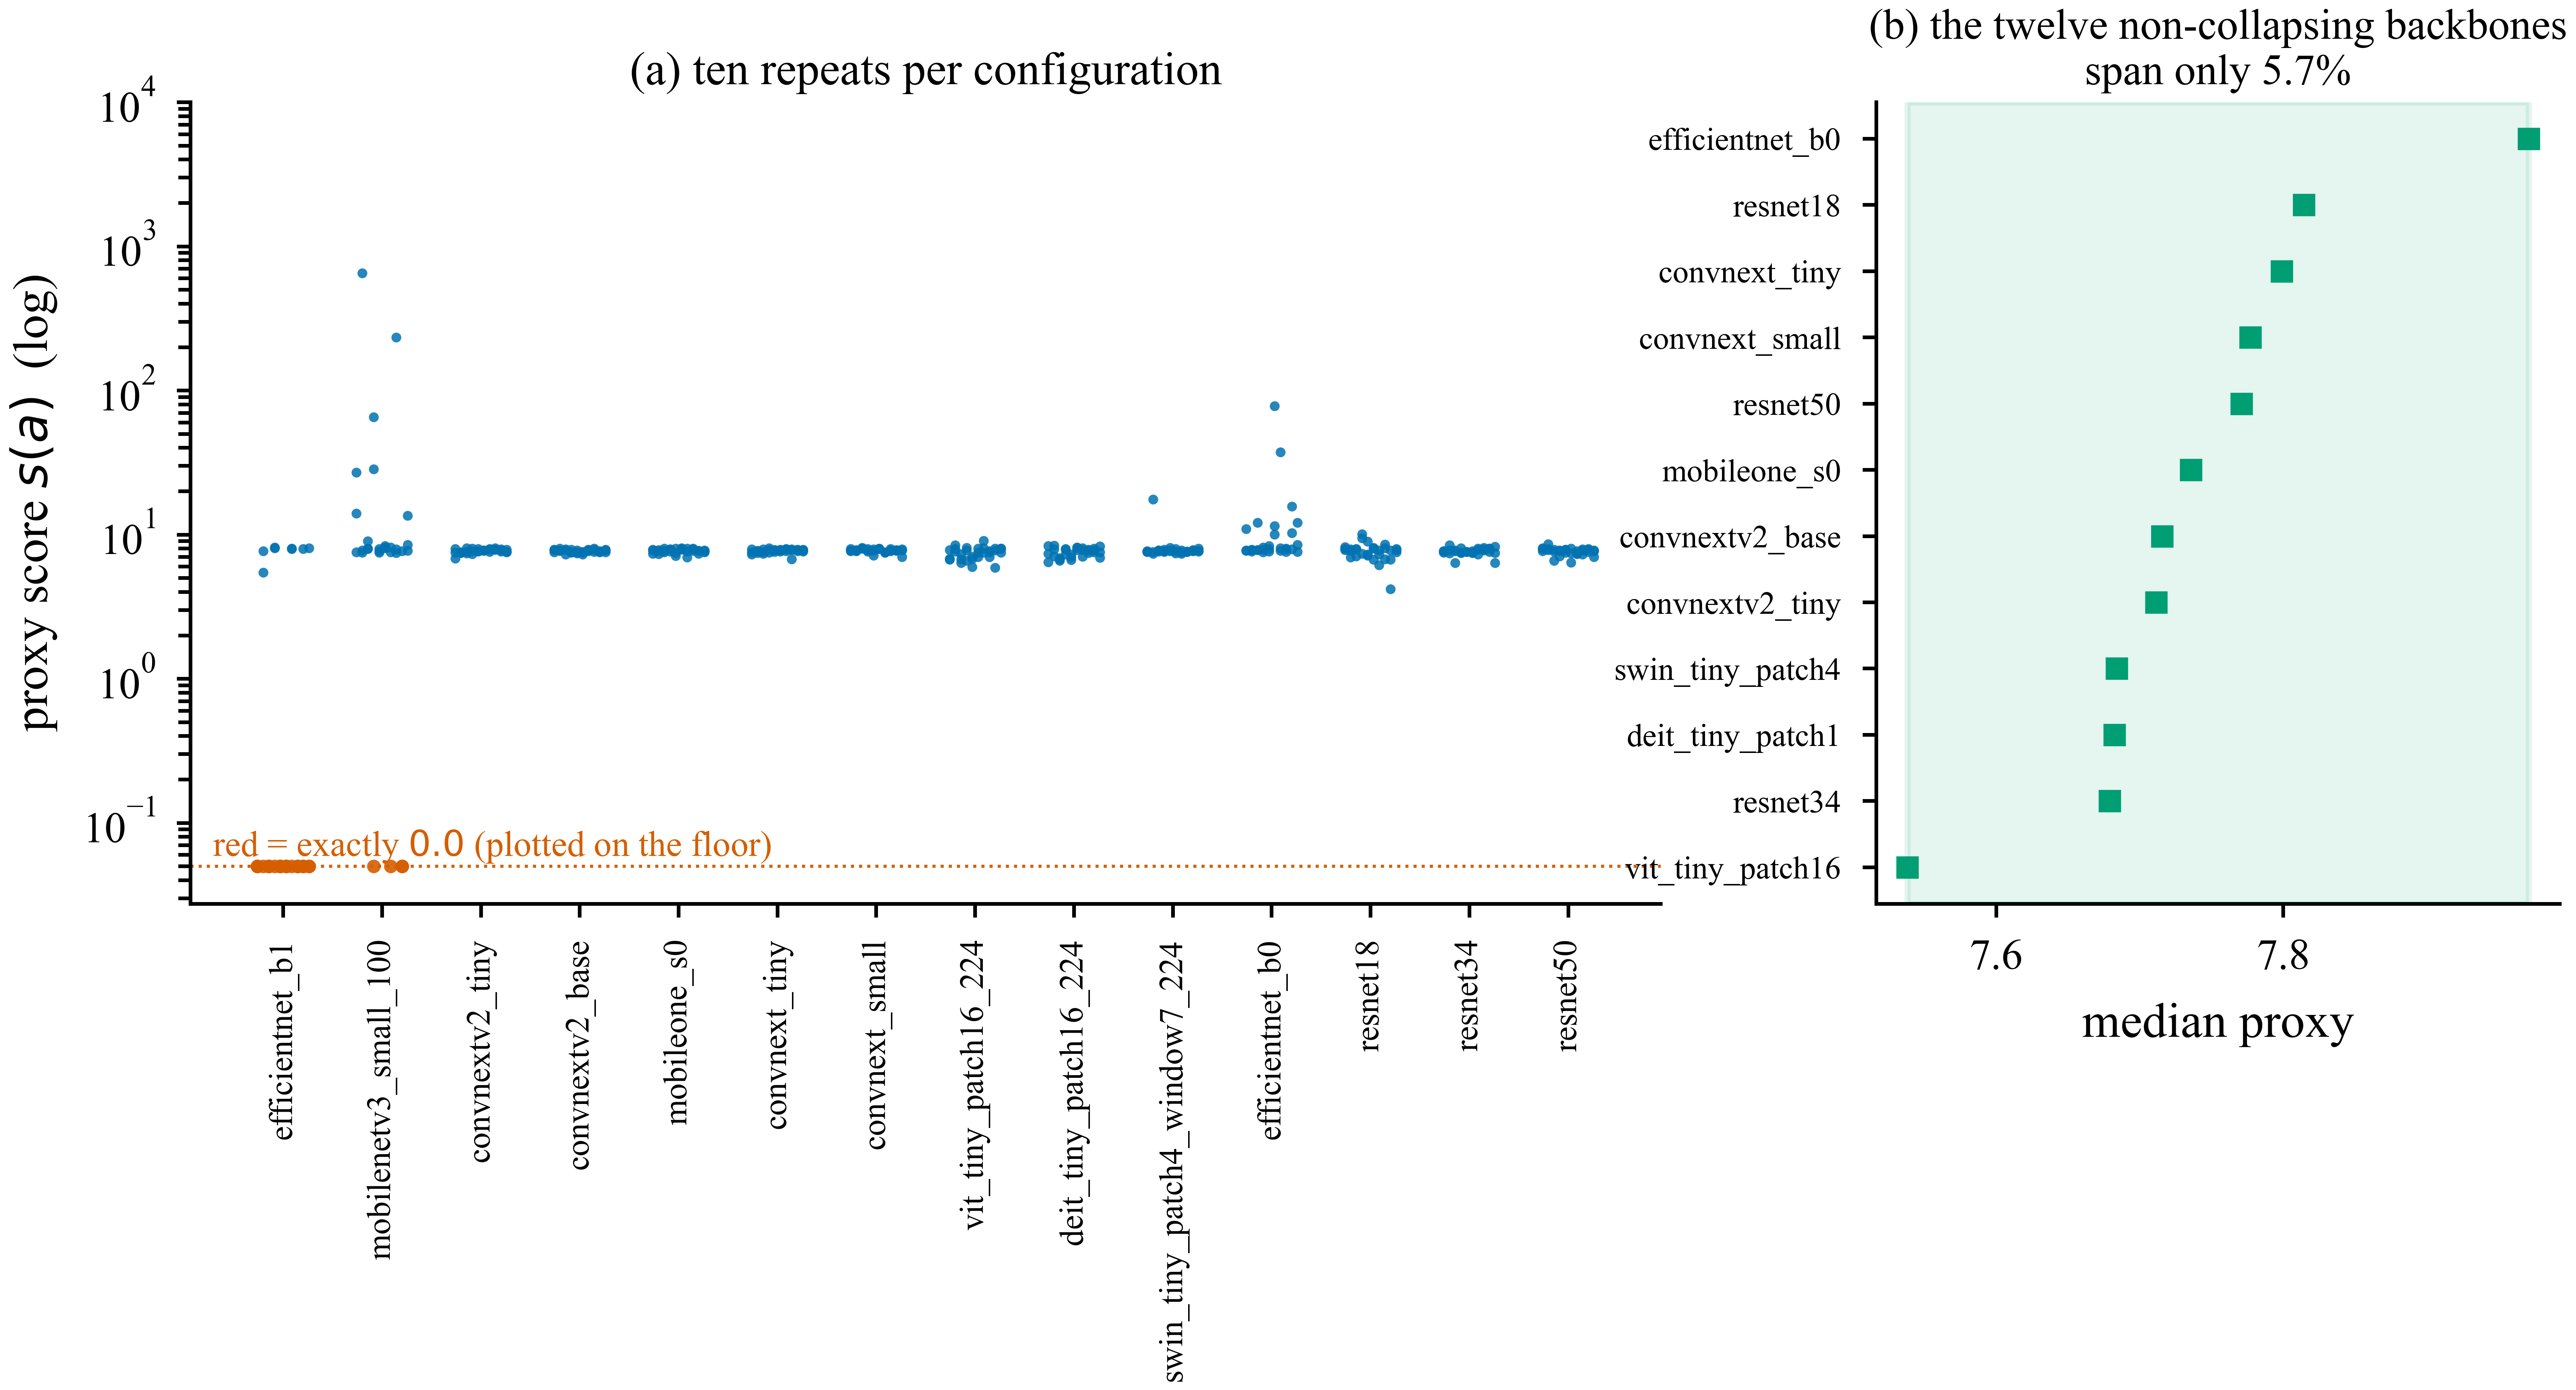
\includegraphics[width=\linewidth]{figures_v2/fig2_proxy_repeatability.png}
\caption{Proxy repeatability. (a) Ten independent evaluations of each of the 42
configurations, on a logarithmic axis. Eleven backbones form a tight band near
$7.6$ (\texttt{efficientnet\_b0} is degenerate-free but sits higher and wider);
\texttt{efficientnet\_b1} and \texttt{mobilenetv3\_small\_100} intermittently
return exactly $0.0$ (marked red, plotted on the axis floor) when their student
diverges. (b) The pooled median of the eleven tight non-collapsing backbones spans
only $5.7\%$, the same order as the within-configuration noise of a single
backbone.}
\label{fig:proxy_repeatability}
\end{figure}

The more consequential number in Table~\ref{tab:proxy_repeats} is the median
column. Across the eleven tight non-collapsing backbones --- CNN and Transformer
families, 2015-era through 2023-era, from ResNets~\cite{he2016deep} to ConvNeXt
V2~\cite{woo2023convnextv2} --- the median proxy spans only $7.54$ to $7.97$, a
range of $5.7\%$, while a single backbone's within-configuration noise is of the
same order ($2$--$12\%$ CV). The proxy contains essentially no
architecture-level signal. Any ranking it produces is not a ranking of
architectures; it is a ranking of which cell happened to be sampled.

\runinhead{Minimising then selects the broken cells.}
This turns a noisy score into a systematically wrong one. A well-behaved
configuration has a lower bound near $7.5$ and can never beat a configuration
that occasionally returns $0.0$. Minimising over the space does not select the
best candidate; it selects the candidate with the heaviest left tail --- and the
left tail is heaviest exactly where training diverged. Consistent with this,
\texttt{efficientnet\_b1}, the backbone that collapses in $73\%$ of evaluations,
is the $\argmin$ reported by the capacity searches of
Section~\ref{subsec:capacity_null} at two of their five parameter bands.

The recorded runs show the same pathology at the same rate. Over every search
result stored in the project --- 19 runs, 834 trials --- $8.0\%$ of trials score
exactly zero, and in \textbf{14 of the 19 runs (74\%)} the plain $\argmin$ over
the recorded results, which is literally what the search returns
(\texttt{min(self.results, key=score)}), points at a zero-score trial
(Table~\ref{tab:degeneracy}). The five capacity-budget searches are all affected,
and were usable only because a later analysis script discards trials scoring
$\le 0$: three different conventions for handling degenerate trials coexist in the
same codebase, the search engine keeping them while the downstream selectors drop
them.

\begin{table}[t]
\centering
\caption{Degenerate trials in the recorded searches, and whether the plain
$\argmin$ lands on one. A trial scoring exactly $0.0$ has had every validation
batch rejected, so the average is \texttt{total}/\texttt{max(count,1)}; because
the search minimises, such a trial wins outright.}
\label{tab:degeneracy}
\resizebox{\columnwidth}{!}{%
\begin{tabular}{lrrl}
\toprule
Run & Trials & Zeros & $\argmin$ config \\
\midrule
\texttt{cap\_budget\_3M}  & 20  & 1  & \texttt{mobilenetv3\_small\_100@128} \\
\texttt{cap\_budget\_6M}  & 40  & 4  & \texttt{mobilenetv3\_small\_100@256} \\
\texttt{cap\_budget\_8M}  & 80  & 11 & \texttt{efficientnet\_b1@256} \\
\texttt{cap\_budget\_13M} & 80  & 13 & \texttt{mobilenetv3\_small\_100@256} \\
\texttt{cap\_budget\_30M} & 80  & 6  & \texttt{efficientnet\_b1@256} \\
\texttt{mvtec\_stage2\_test/bottle} & 100 & 9 & \texttt{efficientnet\_b1@512} \\
\texttt{search\_strategies} (9 runs) & 270 & 23 & 8 of 9 degenerate \\
\midrule
\texttt{stage2} (main search) & 17 & 0 & \texttt{efficientnet\_b0@128} \\
\texttt{stage2\_rtx3090} & 15 & 0 & \texttt{efficientnet\_b0@512} \\
\texttt{stage2\_rtx3090\_100trials} & 39 & 0 & \texttt{efficientnet\_b0@256} \\
\texttt{stage2\_topjournal\_15backbones\_fixed} & 93 & 0 & \texttt{efficientnet\_b0@256} \\
\midrule
\textbf{Total} & \textbf{834} & \textbf{67 (8.0\%)} & \textbf{14 of 19 runs} \\
\bottomrule
\end{tabular}}

\end{table}

\runinhead{A reproducibility caveat.}
The recorded runs predate the current revision of the search engine, and the two
are not numerically identical: the recorded proxy for \texttt{efficientnet\_b0}
spans $0.002$--$0.065$, whereas the current code returns $7.5$--$12.2$ for the
same configuration. We therefore do not claim to reproduce the recorded search;
what the two lines of evidence agree on --- and all we rely on here --- is the
failure mode, its rate ($8.0\%$ against $6.2\%$) and the backbones it afflicts.
The revised engine also returns no zero-score trial in the four runs whose results
the manuscript reports, which is itself evidence of the revision; that the four
happened to select \texttt{efficientnet\_b0}, a backbone that does not collapse,
was in this account luck rather than method
(Section~\ref{subsec:search_vs_random}).

\runinhead{Two further obstacles.}
The proxy's absolute level is not comparable across categories: its median is
$0.110$ on \texttt{capsule}, $0.385$ on \texttt{hazelnut} and $7.56$ on
\texttt{wood}, a span of $68.6\times$, so neither a fixed threshold nor a
cross-category comparison of scores is meaningful --- yet the protocol runs a
single search on one category and transfers the winner to the others. And the
deployment-inert dimension of Section~\ref{subsec:inert}, which cannot change the
detector at all, nevertheless moves the proxy by a median factor of $1.16\times$
across 140 backbone comparisons and by more than $10\times$ at the 90th
percentile. A variable with no deployment meaning is responsible for
order-of-magnitude swings in the ranking.

\subsection{The Searched Axis Has No Measurable Effect on Accuracy}
\label{subsec:capacity_null}

A search that ranks noise could still be worth running if the axis it explores
mattered. We test that directly, by retraining detectors across the whole
parameter range under five mutually exclusive parameter bands, each trained with
the identical protocol (500 epochs, batch size 64, seed 42, ResNet-18 teacher,
reverse distillation). Within each band the search is restricted to backbones
whose deployed size (encoder plus decoder) falls inside the band, and the
best-scoring backbone is trained on all 15 MVTec-AD categories.
Table~\ref{tab:capacity_null} reports the result.

\begin{table}[t]
\centering
\caption{Parameter-capacity bands. Each band restricts the search to backbones
whose deployed size falls inside the band; the selected backbone is then trained
with the identical protocol on all 15 MVTec-AD categories.}
\label{tab:capacity_null}
\resizebox{\columnwidth}{!}{%
\begin{tabular}{llrr}
\toprule
Band & Selected backbone & Params (M) & Mean AUROC (\%) \\
\midrule
0--3M   & MobileNetV3-Small & 2.81  & 82.01 \\
3--6M   & EfficientNet-B0   & 5.41  & 83.14 \\
6--9M   & DeiT-Tiny         & 7.31  & 81.55 \\
9--15M  & ResNet-18         & 13.04 & \textbf{83.25} \\
15--31M & ResNet-50         & 25.77 & 83.08 \\
\bottomrule
\end{tabular}}

\end{table}

Multiplying the parameter budget by $9.2\times$ changes mean AUROC by
$+1.06$ percentage points, and the entire spread across the five bands is
$1.70$ points. The ordering is not monotone: the largest model is worse than the
second largest. All ten pairwise paired $t$-tests across categories are
non-significant (smallest $p = 0.058$).

We then measured the axis directly: all 14 backbones of the search space were
trained on all 15 MVTec-AD categories under the identical protocol, giving 210
detectors, and the resulting matrix was decomposed. A two-way decomposition
attributes \textbf{$0.54\%$} of the variance to the backbone
($F(13,182) = 1.844$, $p = 0.039$), \textbf{$95.32\%$} to the category, and
$4.13\%$ to their interaction, which is the error term in this repeated-measures
design (Figure~\ref{fig:variance}).

The backbone term is statistically significant: with 210 detectors the test has
the power to detect it. That, precisely, is the point. The effect is detectable
\emph{and} negligible. Architecture accounts for $0.54\%$ of the variance in
detection accuracy, against $95.32\%$ for which category is being inspected --- a
factor of $175$. A practitioner choosing between two backbones is moving an
AUROC whose variation is overwhelmingly determined by the object under
inspection rather than by the network.

The ranking says the same thing. Over the 15 categories the 14 backbones span
\begin{figure}[t]
\centering
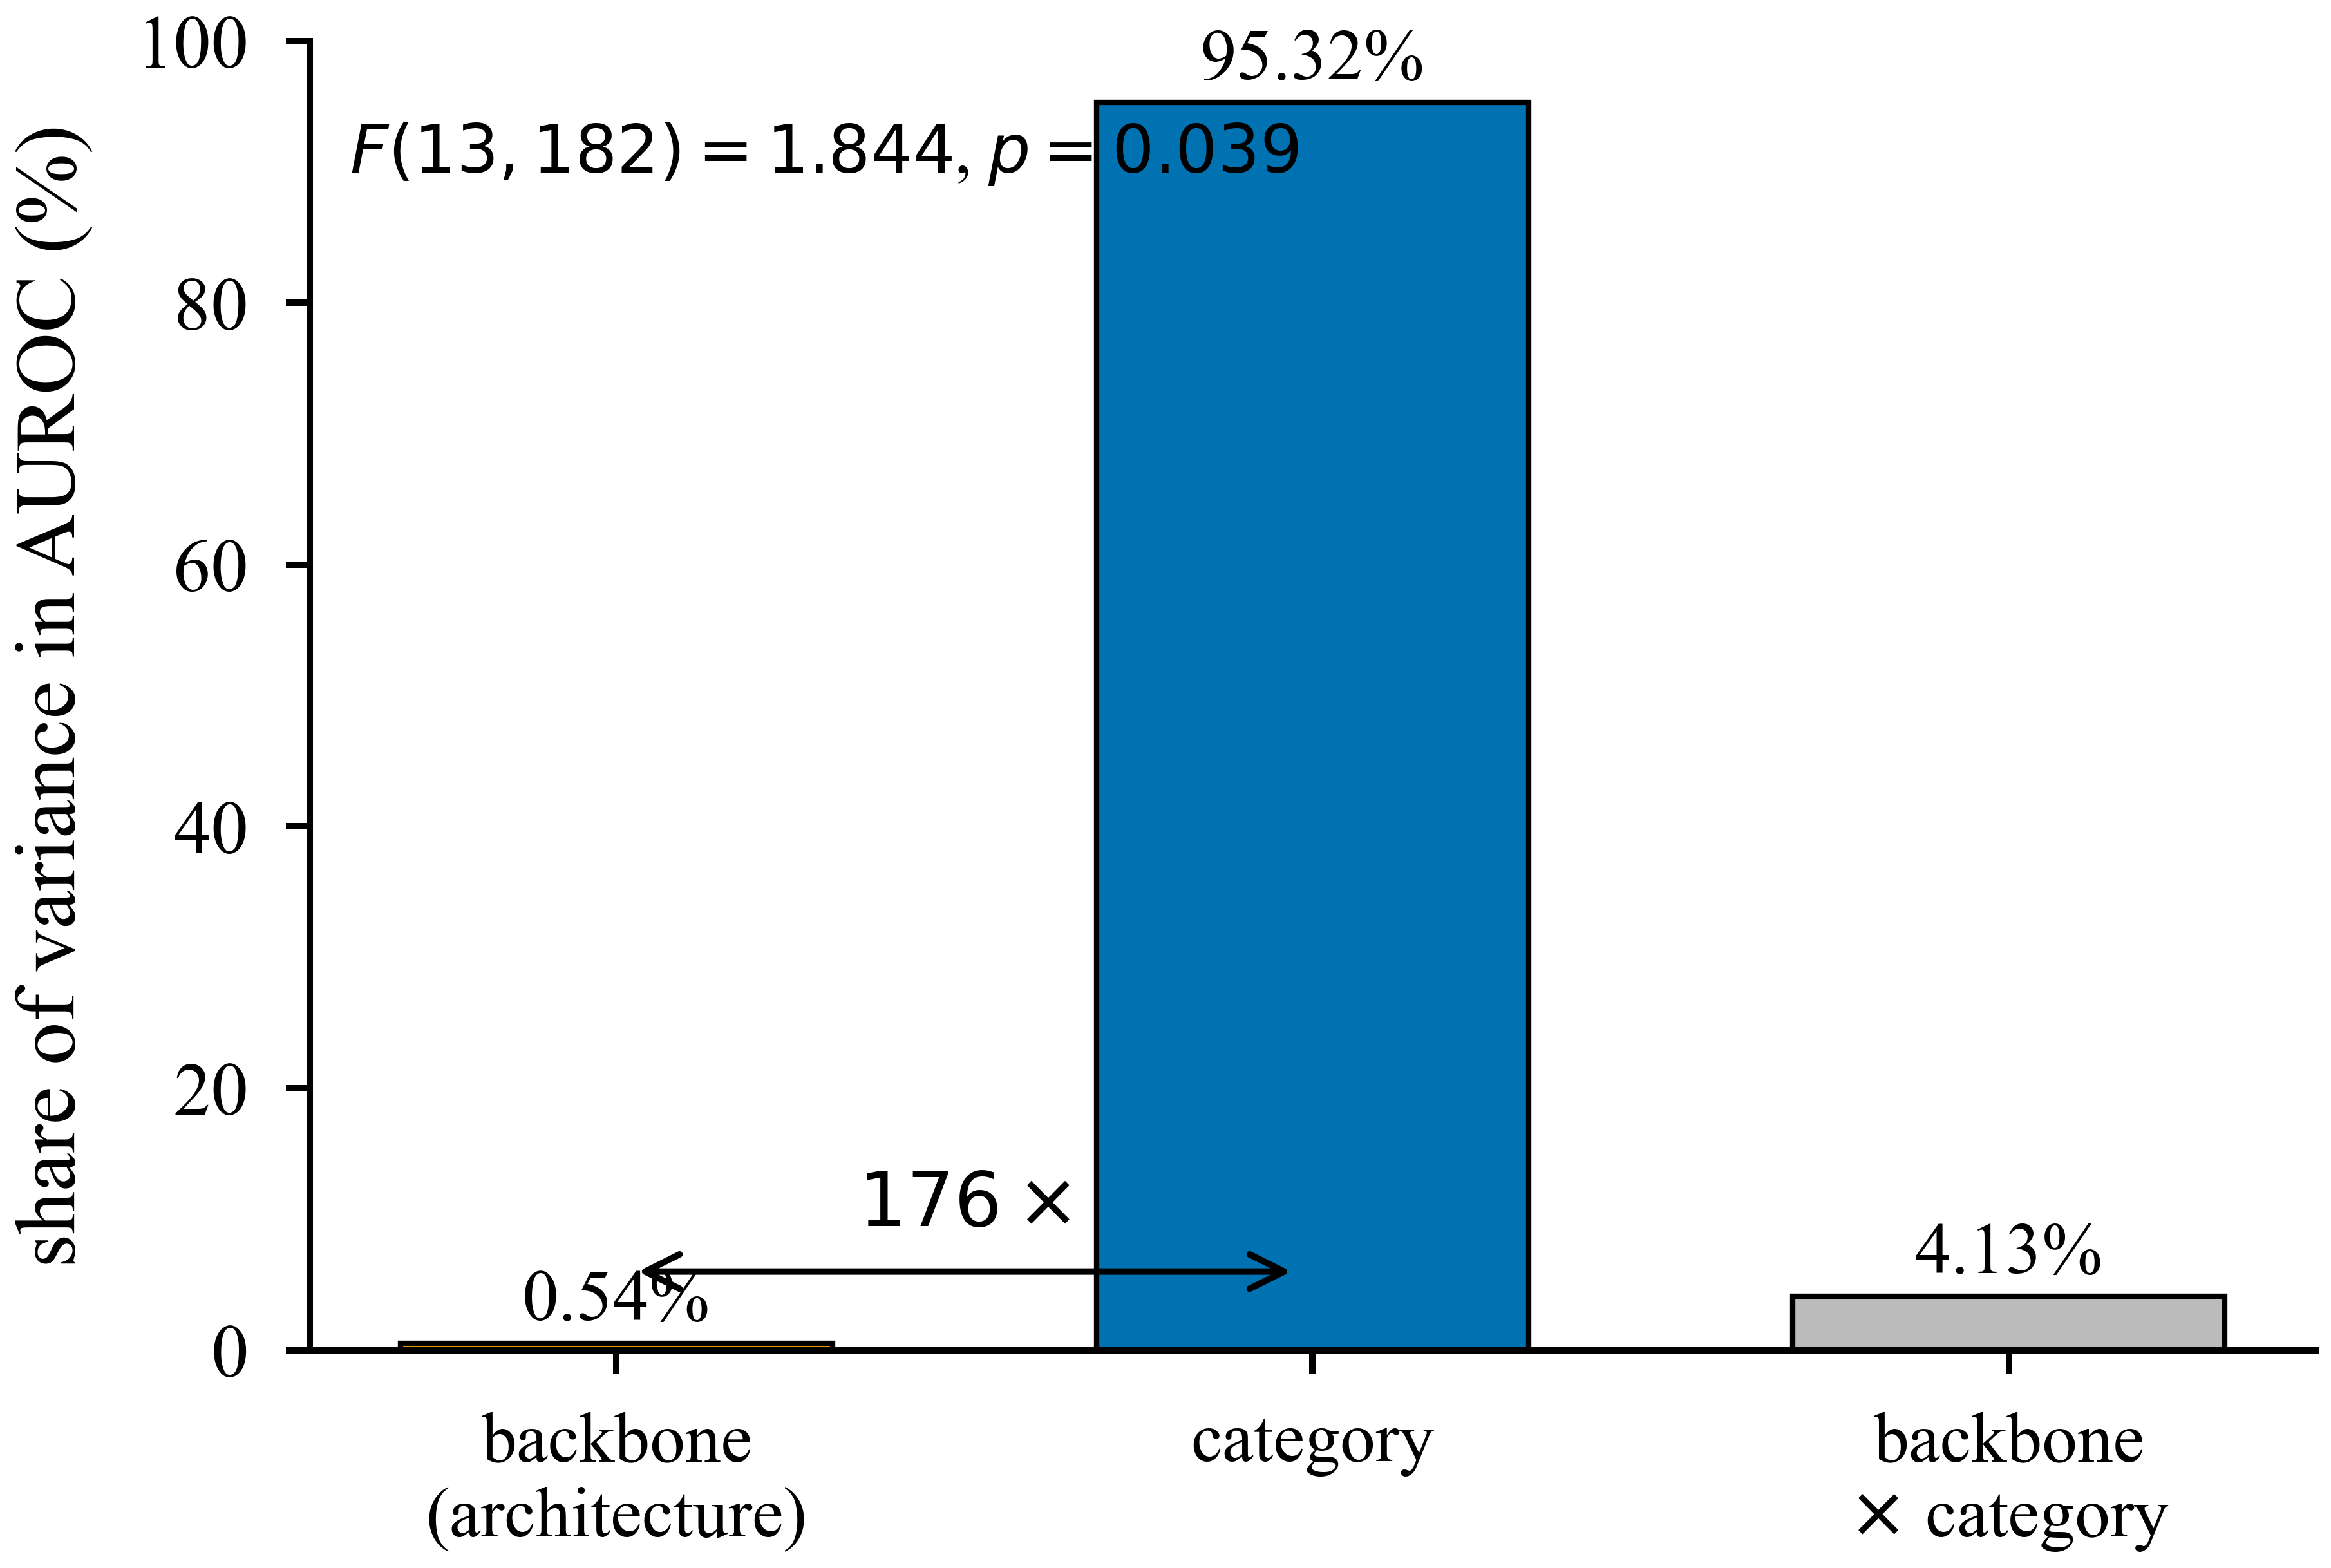
\includegraphics[width=\linewidth]{figures_v2/fig3_variance_decomposition.png}
\caption{Two-way decomposition of the true AUROC over 14 backbones and 15
categories (210 detectors). The backbone effect is statistically detectable and
practically negligible: it accounts for $0.54\%$ of the variance against $95.32\%$
for the category, a factor of $175$.}
\label{fig:variance}
\end{figure}

$3.98$ points of mean AUROC, and the eleven strongest span only $2.43$ points.
The manuscript's selected architecture, \texttt{efficientnet\_b0}, ranks fifth of
fourteen and is statistically indistinguishable from twelve of the thirteen
alternatives; only \texttt{convnextv2\_base} is significantly worse
($-3.11$ points, $p = 0.013$).

\runinhead{The search signal does not predict the target.}
Ranking the 14 backbones by their mean proxy score
(Section~\ref{subsec:proxy_stability}) and comparing that ordering with the true
performance matrix gives a Spearman correlation of \textbf{$-0.12$} ($p = 0.68$)
against the 15-category mean, and \textbf{$+0.02$} ($p = 0.93$) against
performance on \texttt{wood} itself. The search signal is not weakly correlated
with the outcome it exists to select for; on the very category the search is run
on it is indistinguishable from uncorrelated. The consequence is concrete: on
\texttt{wood} the backbone with the highest true AUROC is
\texttt{convnextv2\_base} at $94.74\%$, and across the fifteen categories
\texttt{convnextv2\_base} is the \emph{worst} of the fourteen at $79.36\%$; the
correlation between a backbone's rank on \texttt{wood} and its rank overall is
$-0.24$. The single category the protocol searches on is, if anything, mildly
anti-informative about the rest.

\runinhead{The run-to-run noise is not small.}
Within a fixed (backbone, category) cell the pooled standard deviation across
training seeds is $1.96$ points over 180 residual degrees of freedom, against a
total spread of $3.98$ points across the fourteen backbones. That the two numbers
are of the same order is the whole difficulty of this axis: a single training run
cannot resolve the backbone effect for any individual category, so a comparison
built on one run per configuration is unresolvable in principle rather than merely
imprecise. Section~\ref{subsec:resolvability} turns that into a number.

\runinhead{And the ranking does not transfer.}
Correlating the 14-backbone orderings of every pair of categories (105 pairs)
gives a mean Spearman $\rho = 0.215$, and in $31\%$ of pairs the two categories
\emph{disagree} on the ordering ($\rho < 0$). The protocol searches on a single
category, \texttt{wood}, and applies the winner to all fifteen. Since which
backbone is better depends on the category, a single-category search is not a
noisy estimate of a real quantity; it is an estimate of a quantity that does not
exist independently of the category.

This is the central observation of the paper. Taken with
Sections~\ref{subsec:inert} and~\ref{subsec:proxy_stability}, it says that the
proxy varies enormously across the space while the quantity it is supposed to
predict contributes half a percent of the variance that the category contributes
ninety-five percent of: the search ranks one noisy quantity in order to predict
another that is almost entirely determined by something else.

\subsection{What This Benchmark Design Can Resolve}
\label{subsec:resolvability}

The preceding subsections diagnose the search. This one asks a different
question, about the benchmark rather than about the pipeline: \emph{how small a
difference can the standard evaluation design detect?} The question is forced by
the state of the field. On MVTec-AD, PatchCore reached $99.1\%$ image-level
AUROC~\cite{roth2022patchcore} and the strongest methods reported since reach
$99.6\%$~\cite{liu2023simplenet,guo2025dinomaly}; the contested margin between
successive generations is $0.5$ points, on test sets holding roughly a hundred
images per category. If published comparisons cannot resolve differences of that
size, the ranking they produce is not a ranking of methods.

The 210-detector matrix of Section~\ref{subsec:capacity_null} and the replicated
cells within it supply every quantity the calculation needs. Three numbers come
out of them, all in AUROC points and all computed by
\texttt{proxy\_diag/samplesize\_analysis.py}:

\begin{itemize}
\item $\sigma_{\text{seed}} = 1.96$, the pooled within-cell standard deviation
over training seeds ($90$ cells replicated three times; $180$ residual degrees of
freedom). The distribution of per-cell standard deviations is heavily skewed ---
median $0.58$, maximum $7.74$ --- so the pooled figure is the honest single number
and the median understates the tail.
\item $\sigma_{\text{res}} = 3.30$, the two-way ANOVA residual on the single-seed
matrix. This is the working error for a comparison \emph{between} backbones,
because it also contains the backbone $\times$ category interaction that the
seed-only figure excludes.
\item $\sigma_{\Delta} = 4.12$, the empirical standard deviation of the
per-category difference between two backbones, averaged over the $91$ backbone
pairs. This is what a paired comparison across categories actually sees.
\end{itemize}

Two comparisons follow, and both are unfavourable to the design in common use. On
a \emph{single category}, with two backbones trained independently, the difference
has resolution $\sigma_{\text{seed}} = 1.96$ per arm; detecting the $0.5$-point
contested margin at $80\%$ power with a two-sided test at $\alpha = 0.05$ requires
\textbf{$240$ independent training runs per backbone}. Paired instead across the
fifteen categories the benchmark provides, the minimum detectable difference is
\textbf{$2.98$ points} --- $75\%$ of the entire $3.98$-point spread of the
fourteen backbones, and six times the margin the field argues about. Adding two
more training seeds per cell, as we do here, moves this only to $2.95$ points. To
resolve $0.5$ points by pairing over categories would take $532$ categories; the
benchmark has fifteen.

The requirement is also method-specific, which is a further reason it has to be
reported rather than assumed. Running the same calculation on a PatchCore-style
memory-bank detector, benchmarked through the harness released with this paper,
gives a seed standard deviation of $0.51$ points and a requirement of only $17$
runs per backbone --- a factor of $14$ below the reverse-distillation pipeline
studied here. No single number of runs is therefore sufficient in this field; the
figure belongs with the method it describes.

The implication is not that this benchmark is worthless, but that a
single-category, single-run comparison on it cannot support a claim at the
resolution the literature reports. A backbone ranking must either be averaged over
many categories --- which is what Table~\ref{tab:controlled} does, and why that
table needed $210$ detectors --- or be reported with an explicit statement of what
it can and cannot distinguish. This is also why the architecture effect, though
statistically detectable at $210$ detectors ($p = 0.039$), cannot be
\emph{ranked} reliably by any smaller design: the power that makes the effect
visible is the same power the field's usual single-category design lacks. We adopt
this discipline for the rest of the paper, making every backbone comparison on the
15-category mean and reporting differences smaller than about three points as
unresolved rather than as rankings.

\subsection{Running the Search Selects the Broken Backbones}
\label{subsec:search_vs_random}

The preceding subsections describe a search space that is two thirds inert, a
signal that does not discriminate between architectures and collapses to a score
of exactly zero for two of them, and a target quantity that architecture barely
moves. This subsection asks what they amount to in practice, by simply running the
search. We invoke the search engine's own entry point
(\texttt{NASSearchEngine.search}) with the manuscript's settings --- 100 trials,
three quick training epochs per candidate, uniform sampling from the 42 cells ---
and repeat it with twelve independent seeds. Because the searched feature
dimension cannot reach the detector (Section~\ref{subsec:inert}), the deployed
model depends only on the selected backbone, so the true quality of a run's output
can be read directly off the truth matrix of
Section~\ref{subsec:capacity_null}. Every run returned one of the two backbones
that collapse to zero: eight of the twelve returned \texttt{efficientnet\_b1}
(true rank 12 of 14, $80.43\%$ mean AUROC) and four returned
\texttt{mobilenetv3\_small\_100} (rank 7 of 14, $81.85\%$). None of the other
twelve backbones was ever selected, and only 2 of the 14 backbones and 6 of the 42
configurations appeared at all. Under uniform selection the probability of twelve
runs all landing inside that two-element subset is $7.2\times10^{-11}$. The search
does not merely fail to find a good architecture; it is reliably drawn to the two
configurations that break.

The consequence is quantitative, and it is not marginal
(Figure~\ref{fig:search_vs_random}). Averaged over the twelve
runs the search's output attains \textbf{80.91}\% mean AUROC. Picking a backbone
uniformly at random from the same space gives \textbf{81.65}\% (bootstrap
s.d.\ 0.32 points), and the best backbone in the space gives \textbf{83.34}\%.
The search result sits at the \textbf{1.2th percentile} of the random-selection
distribution --- it is worse than $98.8\%$ of uniform draws --- with a mean true
rank of $10.3$ of $14$ against $7.5$ for random, and it never once selected one of
the four strongest backbones. Replacing the search with a random number generator
would have improved the deployed detector; replacing it with the constant
\texttt{resnet18} would have improved it by $2.4$ points.

The mechanism is the one established in Section~\ref{subsec:proxy_stability}: a
well-behaved configuration is bounded below by roughly $7$--$8$, while the two
collapse-prone backbones return exactly $0.0$ whenever their student diverges, so
minimising a single sample per configuration selects the heaviest left tail in the
space --- and the heaviest left tails belong to the configurations that failed.
More trials make this more certain rather than less, because every additional
sample of a collapse-prone backbone is another chance to return the minimum of the
space. The exclusion is not perfectly clean: in the twelve recorded runs
\texttt{efficientnet\_b0} also returned exactly $0.0$ twice, in $2.5\%$ of its 79
trials, against $82\%$ of 72 for \texttt{efficientnet\_b1} and $22\%$ of 87 for
\texttt{mobilenetv3\_small\_100} in the same runs. The two extremes dominate the
minimum, but no backbone is immune, which is why the fix has to be a filter rather
than a blacklist. Our recommendation therefore follows from the mechanism rather
than from any single run: \textbf{a search whose objective can silently return the
optimum of its own range must filter degenerate evaluations before minimising, and
should report the distribution of its per-configuration scores rather than a
single minimum.}

\runinhead{Why the earlier searches looked successful.}
\begin{figure}[t]
\centering
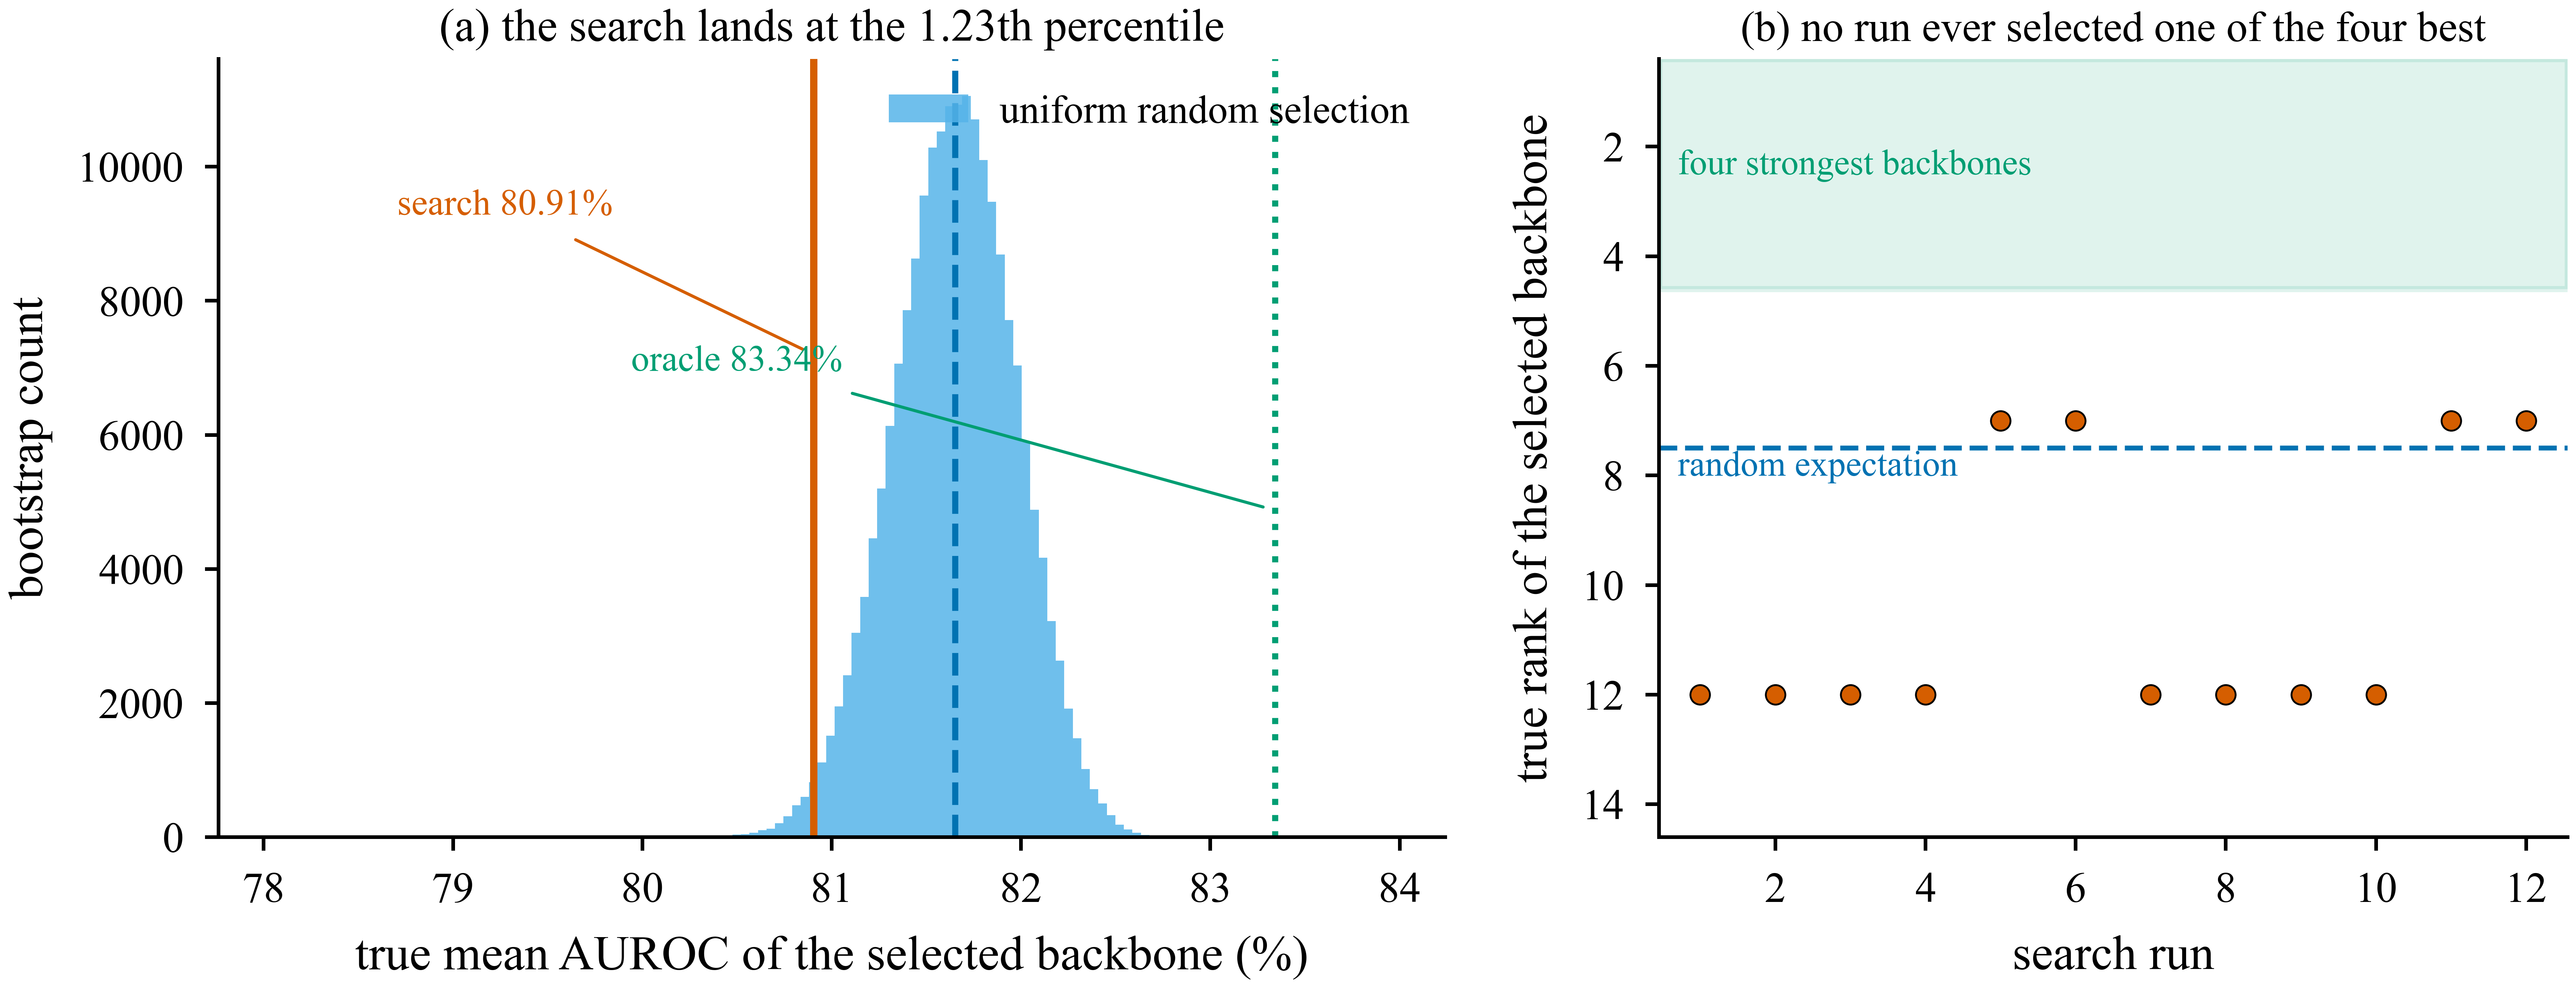
\includegraphics[width=\linewidth]{figures_v2/fig4_search_vs_random.png}
\caption{The search against chance. (a) Bootstrap distribution of the true mean
AUROC obtained by selecting a backbone uniformly at random from the same space,
with the search's output and the oracle marked. The search result sits at the
$1.2$th percentile. (b) True rank of the backbone returned by each of the twelve
runs: the four strongest backbones were never selected.}
\label{fig:search_vs_random}
\end{figure}

The four search runs whose results the manuscript reports selected
\texttt{efficientnet\_b0} (Section~\ref{subsec:inert}), a backbone that collapses
only rarely and never in those four runs. That this is luck rather than method is
the point of Section~\ref{subsec:search_vs_random}, and it is the reason we report
both lines of evidence rather than either alone.
